%\setchapterimage{fig_00.jpg}
\chapter*{Application \arabic{cptApplication} \\ 
Machines Synchrones -- Alternateur
-- \ifprof Corrigé \else Sujet \fi}
\addcontentsline{toc}{section}{Application \arabic{cptApplication} : 
Machines Synchrones -- Alternateur
-- \ifprof Corrigé \else Sujet \fi}

\iflivret \stepcounter{cptApplication} \else
\ifprof  \stepcounter{cptApplication} \else \fi
\fi

\setcounter{question}{0}
\marginnote{Ressources de Philippe Dubois.}


La plaque signalétique d´un alternateur triphasé donne : 
\begin{itemize}
\item $S =\SI{2}{MVA}$; 
\item $\SI{2885}{V}/\SI{5000}{V}$;
\item $\SI{50}{Hz}$ ;
\item $\SI{1500}{tr/min}$.
\end{itemize}

Les enroulements sont couplés en étoile, on mesure la résistance entre deux phases $\indice{R}{mes}=\SI{0,40}{\Omega}$.
On note $L$ l'impédance d'un enroulement d'une phase.
La résistance du rotor $\indice{R}{e}=\SI{10}{\Omega}$.
L’ensemble des pertes fer et mécaniques valent $\SI{65}{kW}$.


Un essai << à vide >> donne une caractéristique d´équation $E = 100I_e$ ou $E$ est la valeur efficace de la fem induite dans un enroulement et $I_e$ est l’intensité du courant d’excitation : $0 < I_e < \SI{50}{A}$.


En charge cet alternateur alimente une installation triphasée équilibrée, inductive, de facteur puissance 0,80, sous une tension efficace nominale $U_n = \SI{5000}{V}$ entre phases. 
L’intensité efficace du courant en ligne est alors $I_n = \SI{200}{A}$ et le courant d´excitation $I_e = \SI{32}{A}$.

\question{Déterminer le nombre de pôles de la machine.}
\ifprof
\begin{marginfigure}
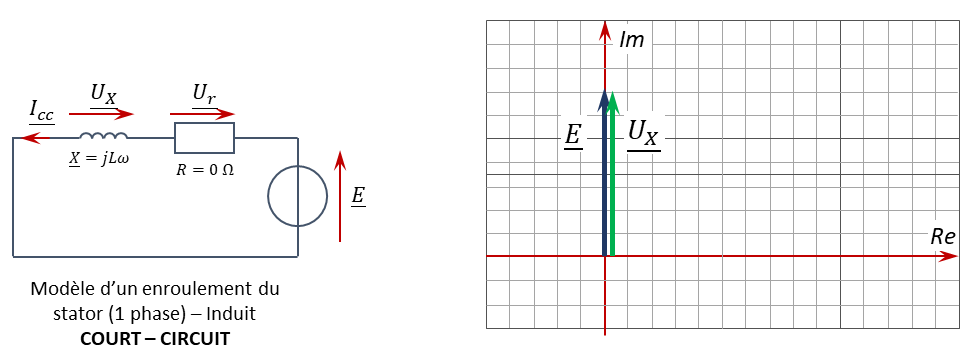
\includegraphics[width=\linewidth]{cor_01}
\end{marginfigure}

\begin{corrige}
À \si{50}{Hz} et 1 paire de pôles, on tourne à  \si{50}{tr/s} soient \si{3000}{tr/min}.  Pour aller à \si{1500}{tr/min} il faut donc 2 paires de pôles. 

On a aussi $N_s = \dfrac{60f}{p}$ $\Rightarrow p =\dfrac{60\times 50}{1500} = 2$.
\end{corrige}
\else
\fi

\question{Rappeler dans quelles conditions est réalisé l'essai << à vide >>.} 
\ifprof
\begin{corrige}
Source ? Moteur entrainé par un MCC à la vitesse de synchronisme ? On mesure une tension simple sur le stator ? et le courant dans le rotor ?
\end{corrige}
\else
\fi

\question{Déterminer la résistance $r$ d'un enroulement statorique.}
\ifprof
\begin{marginfigure}
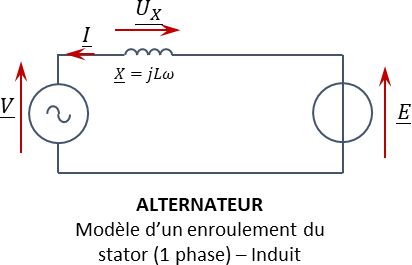
\includegraphics[width=\linewidth]{cor_02}
\end{marginfigure}

\begin{marginfigure}
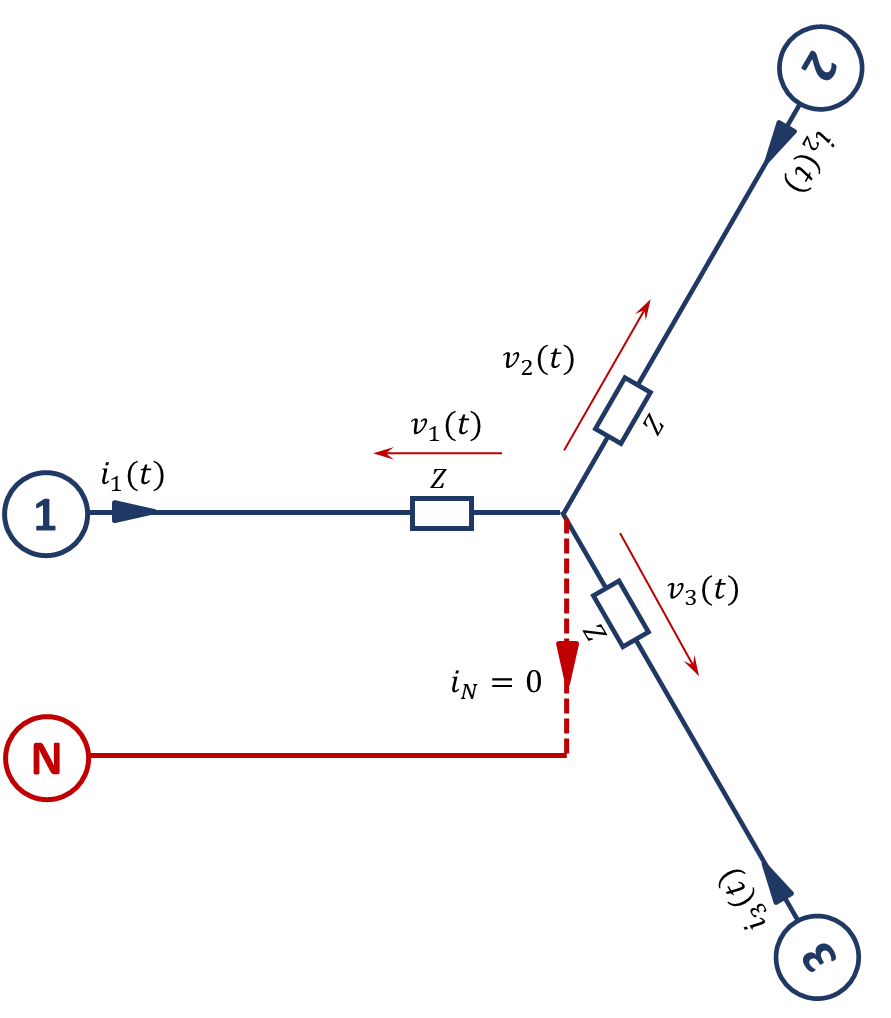
\includegraphics[width=\linewidth]{cor_03}
\end{marginfigure}

\begin{corrige}
Il s'agit ici d'un couplage en étoile. On mesure la résistance entre deux phases. Dans cette configuration, on mesure la tension aux bornes de deux enroulements en série. En notant $r$ la résistance d'un enroulement, on a donc $\indice{R}{mes}=2r$.

\textit{AN :} $r = \SI{0,2}{\Omega}$.

\end{corrige}
\else
\fi



\question{Donner le schéma équivalent d’un enroulement.}
\ifprof
\begin{corrige}
\begin{center}
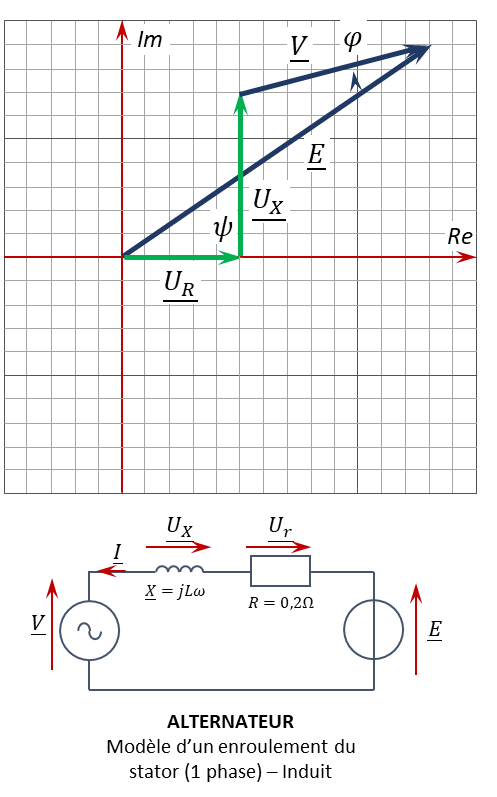
\includegraphics[width=.5\linewidth]{cor_04}
\end{center}
\end{corrige}
\else
\fi


Traiter les questions suivantes pour un fonctionnement << en charge >>.

\question{Tracer le diagramme de Fresnel.}
\ifprof
\begin{corrige}
\end{corrige}
\else
\fi

\question{En faisant l'hypothèse que $r<< L \omega_s$, déterminer la valeur de $L$.}
\ifprof
\begin{corrige}
\end{corrige}
\else
\fi

\question{Calculer la puissance utile, les différentes pertes, la puissance absorbée totale, le rendement et le moment du couple nécessaire pour entrainer la machine synchrone.}
\ifprof
\begin{corrige}
\end{corrige}
\else
\fi

\ifprof
\else
\begin{marginfigure}[-3cm]
\centering
%\includegraphics[width=3cm]{Cy_02_Ch_01_Activation_01_qr}
\end{marginfigure}
\fi




